\documentclass[11pt,a4paper]{article}

\usepackage[margin=0.85in]{geometry}
\usepackage{amsmath,amssymb,amsfonts}
\usepackage{mathtools}
\usepackage{booktabs}
\usepackage{enumitem}
\usepackage{xcolor}
\usepackage{hyperref}
\usepackage{cleveref}
\usepackage{tikz}
\usetikzlibrary{arrows.meta, positioning, shapes.geometric, calc, fit, backgrounds, decorations.pathreplacing}

\definecolor{primaryblue}{RGB}{31, 119, 180}
\definecolor{branchorange}{RGB}{230, 110, 0}
\definecolor{termgreen}{RGB}{44, 160, 44}
\definecolor{fitpurple}{RGB}{130, 80, 175}
\definecolor{batchedteal}{RGB}{0, 135, 145}
\definecolor{daggray}{RGB}{175, 175, 175}
\definecolor{derailred}{RGB}{214, 39, 40}
\definecolor{boxbg}{RGB}{248, 249, 252}

\hypersetup{
    colorlinks=true,
    linkcolor=primaryblue,
    citecolor=primaryblue,
    urlcolor=primaryblue
}

\title{\textbf{Plain-English Guide to the VinePPO Testbed:\\Environments, Transformer Critic, Batched FBI, and Staged FBI}}
\author{Project Overview \& Visual Walkthrough}
\date{\today}

\begin{document}

\maketitle

\section{What This Project Is Doing (Big Picture)}

When training a Large Language Model (LLM) to solve multi-step math or reasoning problems using Reinforcement Learning (RL), we usually only get a reward at the very end of the solution: $R = 1$ if the final answer is right, and $R = 0$ if it is wrong. 

To train the model effectively with PPO (Proximal Policy Optimization), we need a \textbf{Critic} (value function $V_\phi(s_t)$) that can look at an incomplete reasoning chain at step $t$ and estimate: \emph{``What is the probability that the model will eventually reach a correct final answer from this point?''} Once we know the value of every step, we can tell whether a specific reasoning step $a_t$ improved or hurt our chances of success via the step-level advantage:
\[
    \hat{A}(s_t, a_t) = r_t + \gamma V(s_{t+1}) - V(s_t).
\]
Rather than running expensive LLM decoding experiments to study how best to train this critic, this project builds a fast, exact, pure-JAX synthetic testbed where we \textbf{know the exact ground-truth value $V^*(s)$ of every state} via dynamic programming, allowing us to directly measure how fast and accurately different RL value-learning algorithms converge.

\bigskip

\section{The Environments (MRPs / MDPs)}

The codebase models multi-step reasoning using two synthetic Markov environments where observations are sequences of tokens fed into a Transformer, and rewards are sparse and binary ($R \in \{0, 1\}$ at the end of the episode):

\begin{enumerate}[leftmargin=*]
    \item \textbf{Binary Tree MRP (\texttt{envs/tree\_mrp.py}):}
    \begin{itemize}
        \item \textbf{Structure:} A complete binary tree of depth $D$ (e.g., $D=4$ or $D=7$) with $2^{D+1}-1$ states. Starting at the root $s_0$, at each step the trajectory branches Left (\texttt{0}) or Right (\texttt{1}).
        \item \textbf{Rewards \& Dynamics:} Only a small cluster of leaf nodes at depth $D$ are ``correct solutions'' yielding $R = 1$; all other leaves yield $R = 0$. At any internal node where one child subtree contains a correct leaf and the other is a dead end, the base policy picks the correct branch with probability $p$ (e.g., $p = 0.8$) and blunders into the dead-end subtree with probability $1 - p$.
        \item \textbf{Observation:} The sequence of binary choices taken so far, padded to length $D$ (e.g., \texttt{[1, 0, 1, PAD, PAD]}).
    \end{itemize}

    \item \textbf{Procedural Reasoning DAG (\texttt{envs/reasoning\_dag\_env.py}):}
    \begin{itemize}
        \item \textbf{Why a DAG instead of a Tree?} Real reasoning is not a strict tree: different valid chains of thought can reconverge to the same intermediate milestone, and if a model makes a mistake (derails), it can verify/self-correct and get back on track.
        \item \textbf{Hidden Markov State:} Each problem requires completing $M$ sequential \textbf{milestones} within $T$ maximum steps ($T > M$). The true underlying state is tracked by the tuple $(\texttt{prompt\_idx},\, \text{step } t,\, \text{milestone } m \in \{0..M\},\, \texttt{is\_derailed } d \in \{0, 1\})$.
        \item \textbf{Transitions:} At each step, the base policy chooses from $|A|$ discrete action tokens. When on-track ($d=0$), picking a valid advance token increments the milestone ($m \to m+1$, probability $p_{\text{advance}}=0.65$), picking a neutral token keeps $(m, d=0)$, and picking a blunder token derails the trajectory ($d \to 1$, probability $p_{\text{blunder}}=0.15$). Once derailed ($d=1$), normal actions fail to advance $m$; the trajectory can only return to $d=0$ by emitting a special \textbf{self-correction/verification action} (probability $p_{\text{recover}}=0.35$).
        \item \textbf{What the Critic Sees:} Crucially, the network \textbf{never} sees the privileged $(m, d)$ variables. It only sees the raw sequence of emitted token IDs: \texttt{[BOS, PROMPT\_ID, SEP, $a_0$, $a_1$, \dots, $a_{t-1}$, PAD, \dots]}. It must infer which milestone has been reached and whether the chain of thought is currently derailed purely from the token history.
    \end{itemize}
\end{enumerate}

In both environments, an exact backward-induction solver (\texttt{solve\_backward\_induction()}) precomputes the true value $V^*(s)$ and true action advantages $A^*(s, a)$ for every state so we can evaluate the critic's Mean Squared Value Error (MSVE) and Advantage Cosine Similarity at every training step.

\bigskip

\section{The Network (\texttt{transformer.py})}

The critic $V_\phi(s_t)$ is a modern, miniature LLaMA-style causal Transformer (\texttt{TransformerCritic}):
\begin{enumerate}[leftmargin=*]
    \item \textbf{Token Embedding:} Maps the discrete observation sequence (and an optional prepended \texttt{BOS} token) into $d_{\text{model}}$-dimensional vectors (default $d_{\text{model}} = 64$).
    \item \textbf{Causal Transformer Blocks ($N=2$ layers, $H=4$ heads):} Each layer applies Pre-RMSNorm, Multi-Head Causal Self-Attention with Rotary Position Embeddings (RoPE), and a SwiGLU feed-forward network.
    \item \textbf{Last-Valid-Token Pooling:} Extracts the hidden state at the last non-padding token position (which summarizes the entire reasoning prefix up to step $t$).
    \item \textbf{MLP \& Value Head:} Passes that pooled vector through a 2-layer SiLU MLP with RMSNorm and a zero-initialized linear projection head to output a scalar value prediction $V_\phi(s_t) \in \mathbb{R}$.
\end{enumerate}

\bigskip

\section{The Value-Learning Algorithms}

Every algorithm starts an outer training update by rolling out a batch of $B = 64$ primary ``base trajectories'' (chains) $\tau = (s_0, a_0, s_1, \dots, s_T)$, and differs in how it constructs and fits the regression targets $y(s_t)$ for the states along that chain.

\subsection{Algorithm 1: Standard Monte Carlo}
\begin{itemize}[leftmargin=*, itemsep=2pt]
    \item \textbf{How it works:} Generates only the single base trajectory ($K=1$). Every intermediate state $s_t$ along that trajectory is trained to predict the final binary reward $R(s_T) \in \{0, 1\}$ of that single rollout ($y_t^{\text{MC}} = R(s_T)$ for all $t \in \{0, \dots, T\}$).
    \item \textbf{Trade-off:} Cheapest rollout cost ($\mathcal{O}(T)$ transitions per trajectory), but highest variance: the same intermediate state $s_t$ receives target $1$ on one trajectory and $0$ on another.
\end{itemize}

\subsection{Algorithm 2: Vine-Target (Full-Horizon Branching)}
\begin{itemize}[leftmargin=*, itemsep=2pt]
    \item \textbf{How it works:} Inspired by VinePPO, at \emph{every} visited state $s_t$ along the base trajectory, the environment state is cloned $K$ times (e.g., $K=4$) and rolled out \textbf{all the way to the end of the episode ($t \to T$)}. The average terminal reward $\hat{V}_{\text{MC}}(s_t) = \frac{1}{K}\sum_{k=1}^K R(\tau_{t \to T}^{(k)})$ is used as a low-variance target.
    \item \textbf{Optional Precision-Weighted Shrinkage:} Because $\hat{V}_{\text{MC}}(s_t)$ is an average of $K$ Bernoulli trials, its sampling variance is $\hat{\sigma}^2_{\text{MC}}(s_t) = \frac{\hat{V}_{\text{MC}}(1-\hat{V}_{\text{MC}})}{K-1}$. We can optionally blend $\hat{V}_{\text{MC}}(s_t)$ with the current critic prediction $V_\phi(s_t)$ using inverse-variance weights when the critic is already accurate.
    \item \textbf{Trade-off:} Unbiased Monte Carlo targets (zero bootstrapping drift), but requires $\mathcal{O}(K \cdot T^2)$ environment transitions per trajectory because every intermediate branch must be rolled out all the way to horizon $T$.
\end{itemize}

\medskip
\noindent\textbf{The Core Idea of Fitted Backward Induction (FBI) --- 1-Step Branching:}
Instead of rolling out $K$ branches all the way to the end of the episode ($T$), \textbf{Fitted Backward Induction (FBI)} rolls out $K$ parallel branches for \textbf{only 1 step} from each state $s_t$ on the primary chain:
\[
    s_t \xrightarrow{a_t^{(k)} \sim \pi} \big(r_t^{(k)},\; s_{t+1}^{(k)}\big), \qquad k = 1, \dots, K,
\]
reducing the total rollout cost from $\mathcal{O}(K \cdot T^2)$ to $\mathcal{O}(K \cdot T)$. Given critic parameters $\theta$, we approximate the expected 1-step Bellman backup at $s_t$ by averaging over those $K$ children:
\[
    \hat{V}_{\text{branch}}(s_t; \theta) \;=\; \frac{1}{K}\sum_{k=1}^K \Big( r_t^{(k)} + \gamma \, V_\theta\big(s_{t+1}^{(k)}\big) \Big),
\]
where $V_\theta(s_T^{(k)}) \equiv 0$ after a terminal step (so at the penultimate step $t = T-1$, $\hat{V}_{\text{branch}}(s_{T-1}) = \frac{1}{K}\sum_{k=1}^K R(s_T^{(k)})$ is an \textbf{exact} average of terminal rewards with no critic bootstrap).
To optionally blend this 1-step branched backup with longer-horizon returns along the primary chain via $\lambda \in [0, 1]$, we define the branched TD residual $\delta_t^{\text{branch}}(\theta) = \hat{V}_{\text{branch}}(s_t; \theta) - V_\theta(s_t)$ and the general $\lambda$-return target:
\[
    y_t^{(\lambda)}(\theta) \;=\; \hat{V}_{\text{branch}}(s_t; \theta) \;+\; \gamma \lambda \, \hat{A}_{t+1}^{(\lambda)}(\theta), \qquad
    \text{where}\quad \hat{A}_t^{(\lambda)}(\theta) = \delta_t^{\text{branch}}(\theta) + \gamma \lambda \, \hat{A}_{t+1}^{(\lambda)}(\theta) \quad (\hat{A}_T^{(\lambda)} = 0).
\]
When $\lambda = 0$, the target simplifies to pure 1-step backward induction: $y_t^{(0)}(\theta) = \hat{V}_{\text{branch}}(s_t; \theta)$. Depending on \emph{which critic parameters $\theta$} are plugged into $y_t^{(\lambda)}(\theta)$ and \emph{in what order} the critic is trained, we obtain two distinct algorithms: \textbf{Batched FBI} (Algorithm 3) and \textbf{Staged FBI} (Algorithm 4).

\subsection{\texorpdfstring{Algorithm 3: Batched FBI --- $\text{FBI}_{\text{batched}}(\lambda)$}{Algorithm 3: Batched FBI}}

\textbf{Batched FBI} is the simpler, synchronous algorithm (\Cref{fig:batched_fbi_visual}). Within each outer training iteration, it computes all targets across the entire trajectory first using the fixed pre-update critic parameters $\phi_{\text{old}}$, and then fits the network on all timesteps simultaneously:

\begin{enumerate}[leftmargin=*, itemsep=2pt]
    \item \textbf{Step 1 (Rollout Chain + $K$ 1-Step Branches):}
    Roll out the primary chain $\tau = (s_0, s_1, \dots, s_T)$ and, at each state $s_t$ ($t \in \{0, \dots, T-1\}$), sample $K$ independent 1-step transitions $s_t \to s_{t+1}^{(1..K)}$.
    \item \textbf{Step 2 (Compute All Targets Using Fixed $\phi_{\text{old}}$):}
    Freeze the current critic weights $\theta = \phi_{\text{old}}$ and compute the target $y_t$ for every step $t \in \{0, \dots, T-1\}$:
    \[
        y_t \;=\; y_t^{(\lambda)}(\phi_{\text{old}}) \;=\; \hat{V}_{\text{branch}}(s_t; \phi_{\text{old}}) + \gamma \lambda \, \hat{A}_{t+1}^{(\lambda)}(\phi_{\text{old}}), \qquad \forall\, t \in \{0, \dots, T-1\}.
    \]
    \item \textbf{Step 3 (Fit All Timesteps Simultaneously):}
    Collect the full-trajectory dataset $\mathcal{D}_{\text{all}} = \big\{(s_t, y_t)\big\}_{t=0}^{T-1}$ and update $\phi$ by minimizing the mean squared error over all timesteps together for $E$ passes (epochs):
    \[
        \min_\phi \; \mathcal{L}_{\text{batched}}(\phi) \;=\; \frac{1}{T} \sum_{t=0}^{T-1} \Big( V_\phi(s_t) - y_t \Big)^2.
    \]
\end{enumerate}

\subsection{\texorpdfstring{Algorithm 4: Staged FBI --- $\text{FBI}_{\text{staged}}(\lambda)$}{Algorithm 4: Staged FBI}}

\textbf{Why Staged FBI?} In Batched FBI with $\lambda = 0$, the target at step $t$ is $y_t = \frac{1}{K}\sum_{k=1}^K \big(r_t^{(k)} + \gamma V_{\phi_{\text{old}}}(s_{t+1}^{(k)})\big)$. Early in training, before $V_\phi$ has learned the values at step $t+1$, querying the pre-update network $V_{\phi_{\text{old}}}(s_{t+1}^{(k)})$ yields uncalibrated predictions, so it takes at least $T$ separate outer rollout iterations for terminal reward information at step $T$ to propagate all the way back to $s_0$.

\textbf{Staged FBI} eliminates this lag by solving the value function in \textbf{reverse backward-induction order ($t = T-1 \to 0$)} within a single iteration, updating the critic parameters $\phi^{(T-1)} \to \phi^{(T-2)} \to \dots \to \phi^{(0)}$ at step $t+1$ \emph{before} querying them to construct the target at step $t$ (\Cref{fig:staged_fbi_visual}):

\begin{enumerate}[leftmargin=*, itemsep=2pt]
    \item \textbf{Step 1 (Rollout Chain + $K$ 1-Step Branches):}
    Identical to Batched FBI: roll out the primary chain $\tau = (s_0, \dots, s_T)$ and fork $K$ 1-step branches $s_{t+1}^{(1..K)}$ at each state $s_t$.
    \item \textbf{Step 2A (Base Case at the End of the Chain, $t = T-1$):}
    At the penultimate step $t = T-1$, all $K$ 1-step branches land on terminal states $s_T^{(1..K)}$ where exact terminal rewards $R(s_T^{(k)}) \in \{0, 1\}$ are observed directly from the environment. Thus the target $y_{T-1} = \frac{1}{K}\sum_{k=1}^K R(s_T^{(k)})$ (and $y_T = R(s_T)$) requires no critic bootstrapping. Initialize the active training set $\mathcal{D}_{T-1} = \big\{(s_{T-1}, y_{T-1}),\; (s_T, y_T)\big\}$ and run $M$ gradient steps on $\mathcal{D}_{T-1}$ to obtain calibrated terminal-stage parameters $\phi^{(T-1)}$.
    \item \textbf{Step 2B (Backward Induction Loop for $t = T-2 \text{ down to } 0$):}
    Proceeding backward one step at a time from $t = T-2$ down to $0$:
    \begin{itemize}[itemsep=2pt]
        \item \textbf{Compute Target at Step $t$ Using Just-Fitted Parameters $\phi^{(t+1)}$:} Query the critic $V_{\phi^{(t+1)}}$ (which was just trained on step $t+1$) on the $K$ 1-step children of $s_t$:
        \[
            y_t \;=\; y_t^{(\lambda)}\big(\phi^{(t+1)}\big) \;=\; \frac{1}{K}\sum_{k=1}^K \Big( r_t^{(k)} + \gamma \, V_{\phi^{(t+1)}}\big(s_{t+1}^{(k)}\big) \Big) \;+\; \gamma \lambda \, \hat{A}_{t+1}^{(\lambda)}.
        \]
        \item \textbf{Add $(s_t, y_t)$ to Cumulative Active Set $\mathcal{D}_t$:} Because $V_\phi$ is a single shared neural network, training \emph{only} on step $t$ would overwrite what the network just learned at deeper steps $t+1 \dots T$. We therefore keep all resolved steps $[t \dots T]$ in the active set: $\mathcal{D}_t = \mathcal{D}_{t+1} \cup \big\{(s_t, y_t)\big\} = \big\{(s_\tau, y_\tau)\big\}_{\tau = t}^{T}$.
        \item \textbf{Run $M$ Gradient Steps to Obtain $\phi^{(t)}$:} Update the critic from $\phi^{(t+1)}$ to $\phi^{(t)}$ by taking $M$ gradient steps on the cumulative squared loss $\mathcal{L}_t(\phi) = \frac{1}{|\mathcal{D}_t|} \sum_{\tau = t}^{T} \big( V_\phi(s_\tau) - y_\tau \big)^2$, then step backward ($t \leftarrow t - 1$) until the root $t = 0$ is fitted.
    \end{itemize}
\end{enumerate}

\subsection{Head-to-Head Summary: Batched FBI vs.\ Staged FBI}

\begin{table}[ht!]
\centering
\small
\renewcommand{\arraystretch}{1.2}
\resizebox{\textwidth}{!}{%
\begin{tabular}{@{}lll@{}}
\toprule
\textbf{Property} & \textbf{Algorithm 3: Batched FBI} & \textbf{Algorithm 4: Staged FBI} \\ \midrule
\textbf{Rollout Data} & Primary chain + $K$ 1-step branches per state & Primary chain + $K$ 1-step branches per state \\
\textbf{Target Formula at Step $t$} & $y_t = y_t^{(\lambda)}(\phi_{\text{old}})$ (uses fixed pre-update weights) & $y_t = y_t^{(\lambda)}(\phi^{(t+1)})$ (uses weights just fitted at $t+1$) \\
\textbf{Training Objective} & $\frac{1}{T}\sum_{t=0}^{T-1} (V_\phi(s_t) - y_t)^2$ across all $t$ at once & Sequential stages $t = T-1 \to 0$ on resolved set $\mathcal{D}_t = [t \dots T]$ \\
\textbf{Weighting Across Steps} & \textbf{Uniform:} Every step $t$ receives equal weight & \textbf{Bottom-heavy:} Deeper steps $\tau \approx T$ stay in $\mathcal{D}_t$ across more stages \\
\textbf{Key Advantage} & \textbf{Lower final asymptotic error} (uniform weighting) & \textbf{Faster early learning} (rewards propagate $T \to 0$ in 1 iteration) \\ \bottomrule
\end{tabular}%
}
\caption{\textbf{Mathematical comparison of Batched FBI and Staged FBI.}}
\label{tab:batched_vs_staged}
\end{table}

\newpage
\section{Visual Diagram 1: Batched FBI ($\text{FBI}_{\text{batched}}(\lambda)$)}

\vspace{0.15cm}
\begin{figure}[ht!]
\centering
\resizebox{\textwidth}{!}{%
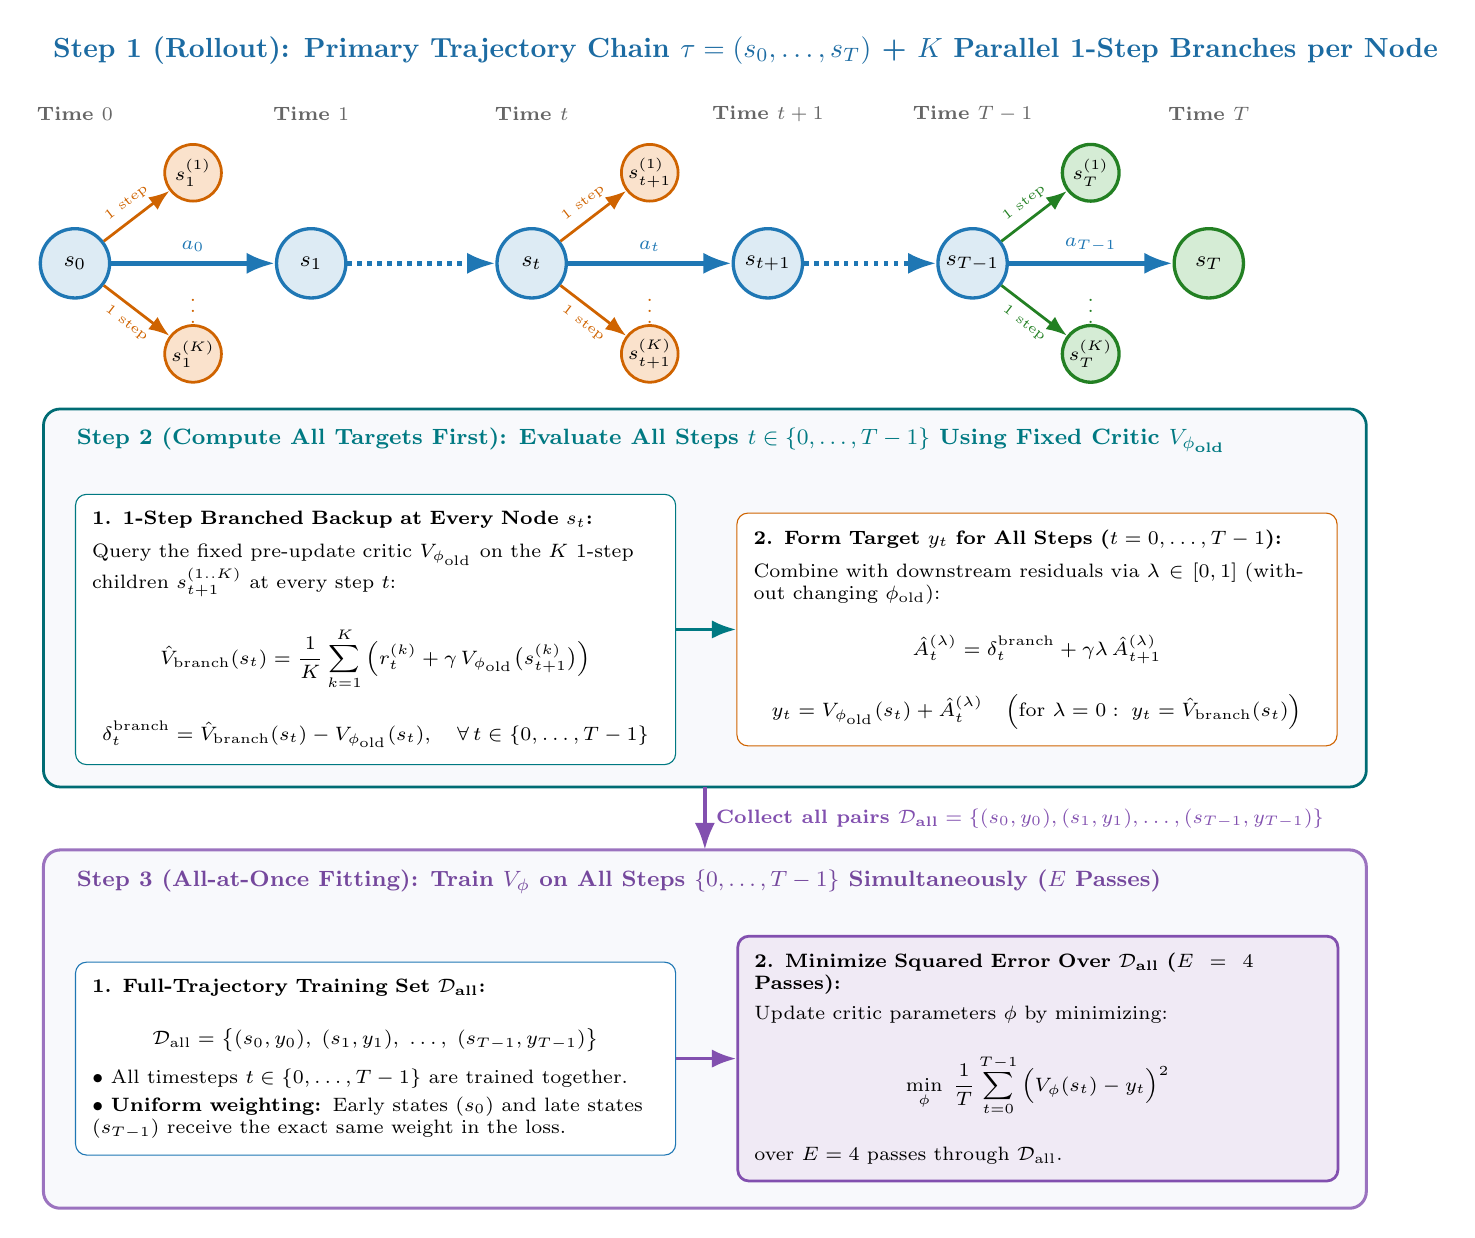
\begin{tikzpicture}[
    >=Latex,
    font=\small,
    chainnode/.style={circle, draw=primaryblue, line width=1.2pt, fill=primaryblue!15, minimum size=8.8mm, inner sep=0pt, font=\footnotesize\bfseries, text=black},
    termnode/.style={circle, draw=termgreen!80!black, line width=1.2pt, fill=termgreen!20, minimum size=8.8mm, inner sep=0pt, font=\footnotesize\bfseries, text=black},
    branchnode/.style={circle, draw=branchorange!90!black, line width=1pt, fill=branchorange!20, minimum size=7.2mm, inner sep=0pt, font=\scriptsize\bfseries, text=black}
]

% =============================================================================
% PANEL 1: THE ROLLOUT CHAIN & PARALLEL 1-STEP BRANCHES
% =============================================================================
\node[anchor=west, font=\normalsize\bfseries, text=primaryblue!90!black] at (-0.4, 10.4)
    {Step 1 (Rollout): Primary Trajectory Chain $\tau = (s_0, \dots, s_T)$ + $K$ Parallel 1-Step Branches per Node};

\begin{scope}[shift={(0, 6.7)}]
    \foreach \x/\step in {0/0, 3.0/1, 5.8/t, 8.8/t+1, 11.4/T-1, 14.4/T} {
        \node[font=\scriptsize\bfseries, text=black!60] at (\x, 2.9) {Time $\step$};
    }

    % Primary Base Trajectory Chain Nodes (blue = non-terminal, green = terminal)
    \node[chainnode] (s0) at (0, 1.0) {$s_0$};
    \node[chainnode] (s1) at (3.0, 1.0) {$s_1$};
    \node[chainnode] (st) at (5.8, 1.0) {$s_t$};
    \node[chainnode] (st1) at (8.8, 1.0) {$s_{t+1}$};
    \node[chainnode] (sTm1) at (11.4, 1.0) {$s_{T-1}$};
    \node[termnode]  (sT) at (14.4, 1.0) {$s_T$};

    % Primary Chain Edges
    \draw[->, primaryblue, line width=1.6pt] (s0) -- node[above, font=\scriptsize] {$a_0$} (s1);
    \draw[->, primaryblue, line width=1.6pt, dotted] (s1) -- (st);
    \draw[->, primaryblue, line width=1.6pt] (st) -- node[above, font=\scriptsize] {$a_t$} (st1);
    \draw[->, primaryblue, line width=1.6pt, dotted] (st1) -- (sTm1);
    \draw[->, primaryblue, line width=1.6pt] (sTm1) -- node[above, font=\scriptsize] {$a_{T-1}$} (sT);

    % K 1-step branches from s_0
    \node[branchnode] (b01) at (1.5, 2.15) {$s_1^{(1)}$};
    \node[branchnode] (b0K) at (1.5, -0.15) {$s_1^{(K)}$};
    \draw[->, branchorange!90!black, line width=1pt] (s0) -- node[above, sloped, font=\tiny] {1 step} (b01);
    \draw[->, branchorange!90!black, line width=1pt] (s0) -- node[below, sloped, font=\tiny] {1 step} (b0K);
    \node[font=\scriptsize, text=branchorange!90!black] at (1.5, 0.5) {$\vdots$};

    % K 1-step branches from s_t
    \node[branchnode] (bt1) at (7.3, 2.15) {$s_{t+1}^{(1)}$};
    \node[branchnode] (btK) at (7.3, -0.15) {$s_{t+1}^{(K)}$};
    \draw[->, branchorange!90!black, line width=1pt] (st) -- node[above, sloped, font=\tiny] {1 step} (bt1);
    \draw[->, branchorange!90!black, line width=1pt] (st) -- node[below, sloped, font=\tiny] {1 step} (btK);
    \node[font=\scriptsize, text=branchorange!90!black] at (7.3, 0.5) {$\vdots$};

    % K 1-step branches from s_{T-1} (landing on terminal states)
    \node[termnode, minimum size=7.2mm, font=\scriptsize\bfseries] (bT1) at (12.9, 2.15) {$s_T^{(1)}$};
    \node[termnode, minimum size=7.2mm, font=\scriptsize\bfseries] (bTK) at (12.9, -0.15) {$s_T^{(K)}$};
    \draw[->, termgreen!80!black, line width=1pt] (sTm1) -- node[above, sloped, font=\tiny] {1 step} (bT1);
    \draw[->, termgreen!80!black, line width=1pt] (sTm1) -- node[below, sloped, font=\tiny] {1 step} (bTK);
    \node[font=\scriptsize, text=termgreen!80!black] at (12.9, 0.5) {$\vdots$};
\end{scope}

% =============================================================================
% PANEL 2: COMPUTE ALL TARGETS AT ONCE USING FIXED \phi_old
% =============================================================================
\begin{scope}[shift={(0, 2.0)}]
    \draw[rounded corners=6pt, draw=batchedteal!80!black, fill=boxbg, line width=1.0pt] (-0.4, -0.95) rectangle (16.4, 3.85);
    \node[anchor=west, font=\footnotesize\bfseries, text=batchedteal!90!black] at (-0.1, 3.45)
        {Step 2 (Compute All Targets First): Evaluate All Steps $t \in \{0, \dots, T-1\}$ Using Fixed Critic $V_{\phi_{\text{old}}}$};

    % Left: 1-Step Branched Backup Box
    \node[draw=batchedteal!90!black, fill=white, rounded corners=4pt, inner sep=6pt, anchor=west, text width=7.2cm, font=\scriptsize] (sync_eval) at (0.0, 1.05) {
        \textbf{1. 1-Step Branched Backup at Every Node $s_t$:}\\[4pt]
        Query the fixed pre-update critic $V_{\phi_{\text{old}}}$ on the $K$ 1-step children $s_{t+1}^{(1..K)}$ at every step $t$:
        \[
            \hat{V}_{\text{branch}}(s_t) = \frac{1}{K}\sum_{k=1}^K \Big(r_t^{(k)} + \gamma \, V_{\phi_{\text{old}}}\big(s_{t+1}^{(k)}\big)\Big)
        \]
        \[
            \delta_t^{\text{branch}} = \hat{V}_{\text{branch}}(s_t) - V_{\phi_{\text{old}}}(s_t), \quad \forall\, t \in \{0, \dots, T-1\}
        \]
    };

    % Right: Lambda Return Target Box
    \node[draw=branchorange!90!black, fill=white, rounded corners=4pt, inner sep=6pt, anchor=west, text width=7.2cm, font=\scriptsize] (sync_gae) at (8.4, 1.05) {
        \textbf{2. Form Target $y_t$ for All Steps ($t = 0, \dots, T-1$):}\\[4pt]
        Combine with downstream residuals via $\lambda \in [0, 1]$ (without changing $\phi_{\text{old}}$):
        \[
            \hat{A}_t^{(\lambda)} = \delta_t^{\text{branch}} + \gamma \lambda \, \hat{A}_{t+1}^{(\lambda)}
        \]
        \[
            y_t = V_{\phi_{\text{old}}}(s_t) + \hat{A}_t^{(\lambda)} \quad \Big(\text{for } \lambda=0:\; y_t = \hat{V}_{\text{branch}}(s_t)\Big)
        \]
    };

    \draw[->, line width=1.3pt, batchedteal!90!black] (sync_eval.east) -- (sync_gae.west);
\end{scope}

% Connector Arrow between Step 2 and Step 3
\draw[->, fitpurple, line width=1.5pt] (8.0, 1.05) -- node[right, font=\scriptsize\bfseries, text=fitpurple] {Collect all pairs $\mathcal{D}_{\text{all}} = \{(s_0, y_0), (s_1, y_1), \dots, (s_{T-1}, y_{T-1})\}$} (8.0, 0.25);

% =============================================================================
% PANEL 3: FIT ALL STEPS SIMULTANEOUSLY
% =============================================================================
\begin{scope}[shift={(0, -3.4)}]
    \draw[rounded corners=6pt, draw=fitpurple!80, fill=boxbg, line width=1.1pt] (-0.4, -0.9) rectangle (16.4, 3.65);
    \node[anchor=west, font=\footnotesize\bfseries, text=fitpurple!90!black] at (-0.1, 3.25)
        {Step 3 (All-at-Once Fitting): Train $V_\phi$ on All Steps $\{0, \dots, T-1\}$ Simultaneously ($E$ Passes)};

    % Left: Full-Trajectory Dataset
    \node[draw=primaryblue, fill=white, rounded corners=4pt, inner sep=6pt, anchor=west, text width=7.2cm, font=\scriptsize] (all_buffer) at (0.0, 1.0) {
        \textbf{1. Full-Trajectory Training Set $\mathcal{D}_{\text{all}}$:}\\[3pt]
        \[
            \mathcal{D}_{\text{all}} = \big\{(s_0, y_0),\; (s_1, y_1),\; \dots,\; (s_{T-1}, y_{T-1})\big\}
        \]
        $\bullet$ All timesteps $t \in \{0, \dots, T-1\}$ are trained together.\\[2pt]
        $\bullet$ \textbf{Uniform weighting:} Early states ($s_0$) and late states ($s_{T-1}$) receive the exact same weight in the loss.
    };

    % Right: Simultaneous Loss Minimization
    \node[draw=fitpurple, fill=fitpurple!12, rounded corners=4pt, line width=1pt, inner sep=6pt, anchor=west, text width=7.2cm, font=\scriptsize] (epochs_box) at (8.4, 1.0) {
        \textbf{2. Minimize Squared Error Over $\mathcal{D}_{\text{all}}$ ($E = 4$ Passes):}\\[3pt]
        Update critic parameters $\phi$ by minimizing:
        \[
            \min_\phi \; \frac{1}{T} \sum_{t=0}^{T-1} \Big( V_\phi(s_t) - y_t \Big)^2
        \]
        over $E = 4$ passes through $\mathcal{D}_{\text{all}}$.
    };

    \draw[->, line width=1.3pt, fitpurple] (all_buffer.east) -- (epochs_box.west);
\end{scope}

\end{tikzpicture}%
}
\caption{\textbf{Algorithm 3: Batched FBI ($\text{FBI}_{\text{batched}}(\lambda)$).} \textbf{Top (Step 1):} Roll out the primary chain $\tau = (s_0, \dots, s_T)$ (blue/green circles) and fork $K$ parallel 1-step branches $s_{t+1}^{(1..K)}$ (orange/green circles) from each visited state $s_t$. \textbf{Middle (Step 2):} Using the fixed pre-update critic $V_{\phi_{\text{old}}}$, compute the targets $y_0, \dots, y_{T-1}$ for all steps first. \textbf{Bottom (Step 3):} Train $V_\phi$ on all steps $\{0, \dots, T-1\}$ simultaneously for $E=4$ passes.}
\label{fig:batched_fbi_visual}
\end{figure}

\newpage
\section{Visual Diagram 2: Staged FBI ($\text{FBI}_{\text{staged}}(\lambda)$)}

\vspace{0.15cm}
\begin{figure}[ht!]
\centering
\resizebox{\textwidth}{!}{%
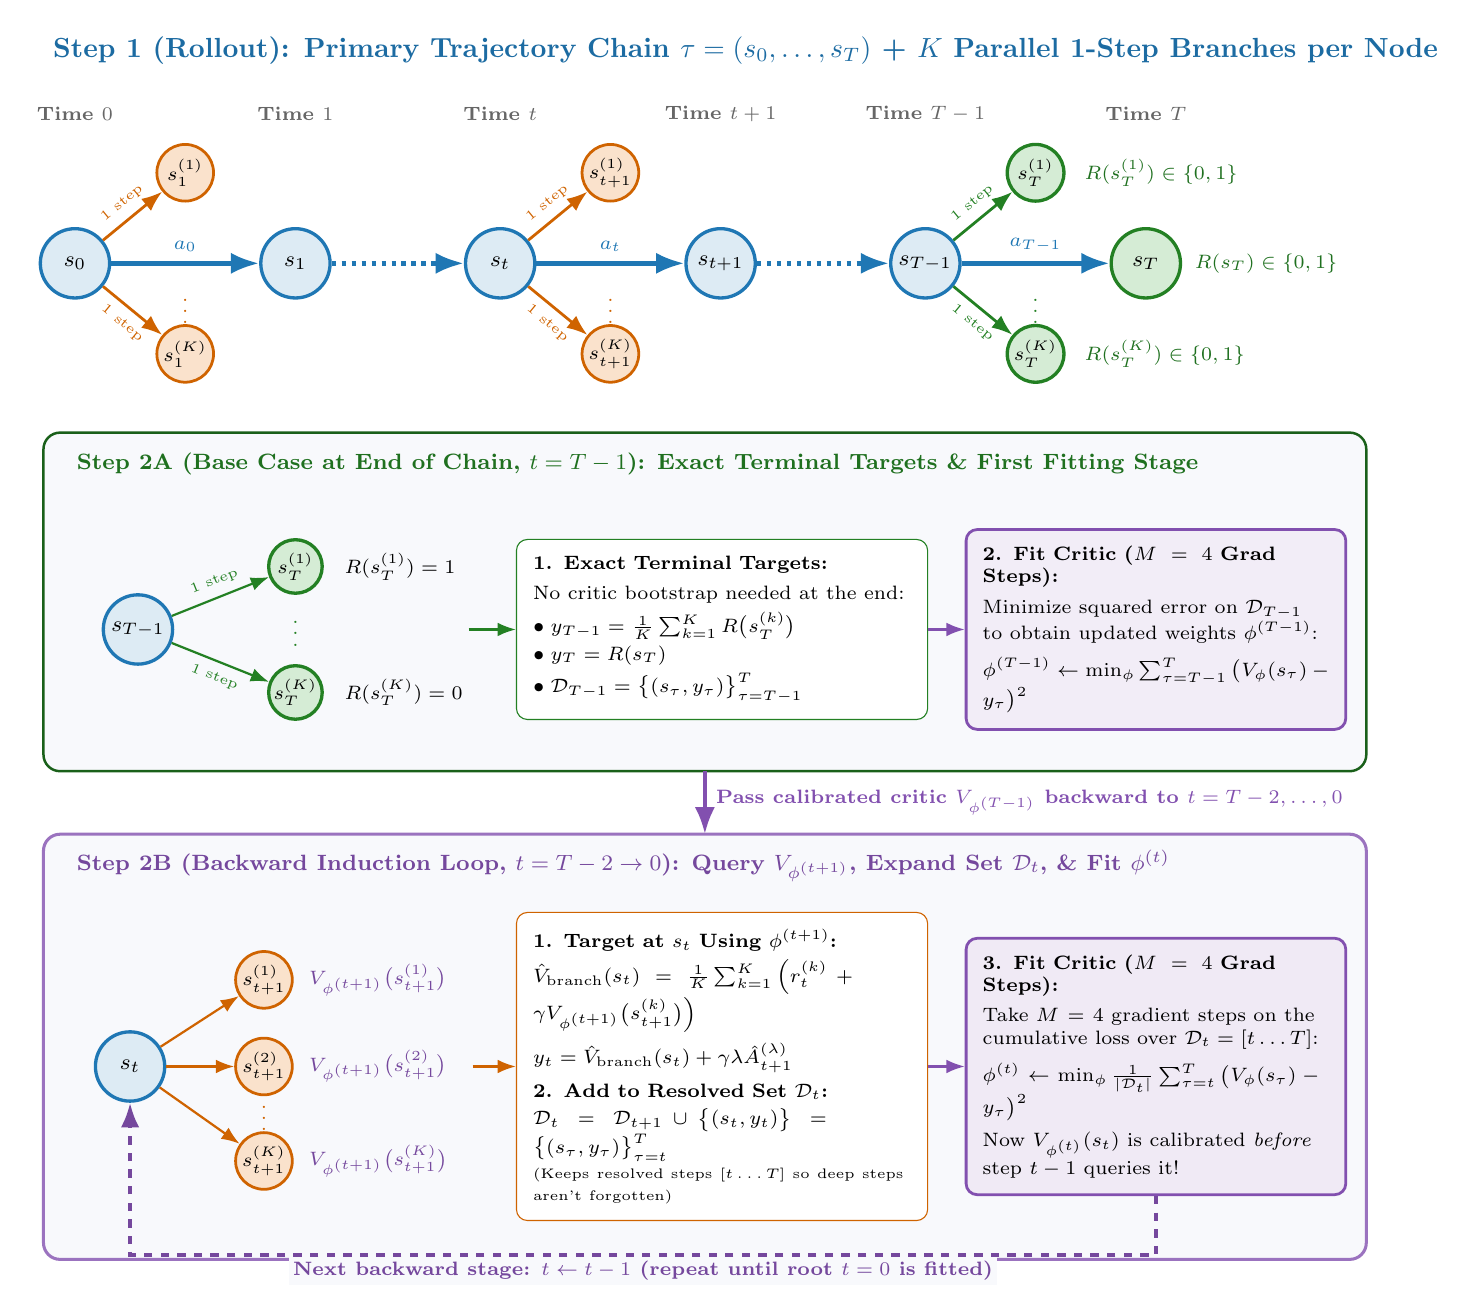
\begin{tikzpicture}[
    >=Latex,
    font=\small,
    chainnode/.style={circle, draw=primaryblue, line width=1.2pt, fill=primaryblue!15, minimum size=8.8mm, inner sep=0pt, font=\footnotesize\bfseries, text=black},
    termnode/.style={circle, draw=termgreen!80!black, line width=1.2pt, fill=termgreen!20, minimum size=8.8mm, inner sep=0pt, font=\footnotesize\bfseries, text=black},
    branchnode/.style={circle, draw=branchorange!90!black, line width=1pt, fill=branchorange!20, minimum size=7.2mm, inner sep=0pt, font=\scriptsize\bfseries, text=black}
]

% =============================================================================
% PANEL 1: THE ROLLOUT CHAIN & PARALLEL 1-STEP FORKS
% =============================================================================
\node[anchor=west, font=\normalsize\bfseries, text=primaryblue!90!black] at (-0.4, 10.4)
    {Step 1 (Rollout): Primary Trajectory Chain $\tau = (s_0, \dots, s_T)$ + $K$ Parallel 1-Step Branches per Node};

\begin{scope}[shift={(0, 6.7)}]
    \foreach \x/\step in {0/0, 2.8/1, 5.4/t, 8.2/t+1, 10.8/T-1, 13.6/T} {
        \node[font=\scriptsize\bfseries, text=black!60] at (\x, 2.9) {Time $\step$};
    }

    % Primary Base Trajectory Chain Nodes
    \node[chainnode] (s0) at (0, 1.0) {$s_0$};
    \node[chainnode] (s1) at (2.8, 1.0) {$s_1$};
    \node[chainnode] (st) at (5.4, 1.0) {$s_t$};
    \node[chainnode] (st1) at (8.2, 1.0) {$s_{t+1}$};
    \node[chainnode] (sTm1) at (10.8, 1.0) {$s_{T-1}$};
    \node[termnode]  (sT) at (13.6, 1.0) {$s_T$};

    % Primary Chain Edges
    \draw[->, primaryblue, line width=1.6pt] (s0) -- node[above, font=\scriptsize] {$a_0$} (s1);
    \draw[->, primaryblue, line width=1.6pt, dotted] (s1) -- (st);
    \draw[->, primaryblue, line width=1.6pt] (st) -- node[above, font=\scriptsize] {$a_t$} (st1);
    \draw[->, primaryblue, line width=1.6pt, dotted] (st1) -- (sTm1);
    \draw[->, primaryblue, line width=1.6pt] (sTm1) -- node[above, font=\scriptsize] {$a_{T-1}$} (sT);

    % K 1-step branches at s_0
    \node[branchnode] (b01) at (1.4, 2.15) {$s_1^{(1)}$};
    \node[branchnode] (b0K) at (1.4, -0.15) {$s_1^{(K)}$};
    \draw[->, branchorange!90!black, line width=1pt] (s0) -- node[above, sloped, font=\tiny] {1 step} (b01);
    \draw[->, branchorange!90!black, line width=1pt] (s0) -- node[below, sloped, font=\tiny] {1 step} (b0K);
    \node[font=\scriptsize, text=branchorange!90!black] at (1.4, 0.5) {$\vdots$};

    % K 1-step branches at intermediary node s_t
    \node[branchnode] (bt1) at (6.8, 2.15) {$s_{t+1}^{(1)}$};
    \node[branchnode] (btK) at (6.8, -0.15) {$s_{t+1}^{(K)}$};
    \draw[->, branchorange!90!black, line width=1pt] (st) -- node[above, sloped, font=\tiny] {1 step} (bt1);
    \draw[->, branchorange!90!black, line width=1pt] (st) -- node[below, sloped, font=\tiny] {1 step} (btK);
    \node[font=\scriptsize, text=branchorange!90!black] at (6.8, 0.5) {$\vdots$};

    % K 1-step branches at penultimate node s_{T-1} (landing on terminal leaves!)
    \node[termnode, minimum size=7.2mm, font=\scriptsize\bfseries] (bT1) at (12.2, 2.15) {$s_T^{(1)}$};
    \node[termnode, minimum size=7.2mm, font=\scriptsize\bfseries] (bTK) at (12.2, -0.15) {$s_T^{(K)}$};
    \draw[->, termgreen!80!black, line width=1pt] (sTm1) -- node[above, sloped, font=\tiny] {1 step} (bT1);
    \draw[->, termgreen!80!black, line width=1pt] (sTm1) -- node[below, sloped, font=\tiny] {1 step} (bTK);
    \node[font=\scriptsize, text=termgreen!80!black] at (12.2, 0.5) {$\vdots$};

    % Terminal reward labels
    \node[anchor=west, font=\scriptsize, text=termgreen!70!black] at (12.7, 2.15) {$R(s_T^{(1)}) \in \{0,1\}$};
    \node[anchor=west, font=\scriptsize, text=termgreen!70!black] at (14.1, 1.0) {$R(s_T) \in \{0,1\}$};
    \node[anchor=west, font=\scriptsize, text=termgreen!70!black] at (12.7, -0.15) {$R(s_T^{(K)}) \in \{0,1\}$};
\end{scope}

% =============================================================================
% PANEL 2: INITIAL BASE CASE (END OF THE CHAIN: t = T - 1)
% =============================================================================
\begin{scope}[shift={(0, 2.3)}]
    \draw[rounded corners=6pt, draw=termgreen!60!black, fill=boxbg, line width=0.9pt] (-0.4, -1.05) rectangle (16.4, 3.25);
    \node[anchor=west, font=\footnotesize\bfseries, text=termgreen!70!black] at (-0.1, 2.85)
        {Step 2A (Base Case at End of Chain, $t = T-1$): Exact Terminal Targets \& First Fitting Stage};

    % Mini diagram of s_{T-1} -> leaves
    \node[chainnode] (init_sTm1) at (0.8, 0.75) {$s_{T-1}$};
    \node[termnode, minimum size=6.8mm, font=\scriptsize] (init_b1) at (2.8, 1.55) {$s_T^{(1)}$};
    \node[termnode, minimum size=6.8mm, font=\scriptsize] (init_bK) at (2.8, -0.05) {$s_T^{(K)}$};
    \node[font=\scriptsize, text=termgreen!80!black] at (2.8, 0.8) {$\vdots$};
    \draw[->, termgreen!80!black, thick] (init_sTm1) -- node[above, sloped, font=\tiny] {1 step} (init_b1);
    \draw[->, termgreen!80!black, thick] (init_sTm1) -- node[below, sloped, font=\tiny] {1 step} (init_bK);

    \node[anchor=west, font=\scriptsize] at (3.3, 1.55) {$R(s_T^{(1)}) = 1$};
    \node[anchor=west, font=\scriptsize] at (3.3, -0.05) {$R(s_T^{(K)}) = 0$};

    % Target box
    \node[draw=termgreen!80!black, fill=white, rounded corners=4pt, inner sep=6pt, anchor=west, text width=4.8cm, font=\scriptsize] (anchor_eq) at (5.6, 0.75) {
        \textbf{1. Exact Terminal Targets:}\\[3pt]
        No critic bootstrap needed at the end:\\[2pt]
        $\bullet\; y_{T-1} = \frac{1}{K}\sum_{k=1}^K R\big(s_T^{(k)}\big)$\\[2pt]
        $\bullet\; y_T = R(s_T)$\\[2pt]
        $\bullet\; \mathcal{D}_{T-1} = \big\{(s_\tau, y_\tau)\big\}_{\tau=T-1}^{T}$
    };

    % Fitting rounds box
    \node[draw=fitpurple, fill=fitpurple!10, rounded corners=4pt, line width=1pt, inner sep=6pt, anchor=west, text width=4.4cm, font=\scriptsize] (fit_init) at (11.3, 0.75) {
        \textbf{2. Fit Critic ($M = 4$ Grad Steps):}\\[3pt]
        Minimize squared error on $\mathcal{D}_{T-1}$ to obtain updated weights $\phi^{(T-1)}$:\\[4pt]
        $\phi^{(T-1)} \leftarrow \min_\phi \sum_{\tau=T-1}^{T} \big(V_\phi(s_\tau) - y_\tau\big)^2$
    };

    \draw[->, thick, termgreen!80!black] (5.0, 0.75) -- (anchor_eq.west);
    \draw[->, thick, fitpurple] (anchor_eq.east) -- (fit_init.west);
\end{scope}

% Backward Loop Connector Arrow between Step 2A and Step 2B
\draw[->, fitpurple, line width=1.5pt] (8.0, 1.25) -- node[right, font=\scriptsize\bfseries, text=fitpurple] {Pass calibrated critic $V_{\phi^{(T-1)}}$ backward to $t = T-2, \dots, 0$} (8.0, 0.45);

% =============================================================================
% PANEL 3: THE INDUCTIVE LOOP AT INTERMEDIARY NODE s_t (REPEATED FOR t = T-2 .. 0)
% =============================================================================
\begin{scope}[shift={(0, -3.7)}]
    \draw[rounded corners=6pt, draw=fitpurple!80, fill=boxbg, line width=1.1pt] (-0.4, -1.25) rectangle (16.4, 4.15);
    \node[anchor=west, font=\footnotesize\bfseries, text=fitpurple!90!black] at (-0.1, 3.75)
        {Step 2B (Backward Induction Loop, $t = T-2 \to 0$): Query $V_{\phi^{(t+1)}}$, Expand Set $\mathcal{D}_t$, \& Fit $\phi^{(t)}$};

    % Left: Intermediary node s_t and its K parallel 1-step children
    \node[chainnode] (loop_st) at (0.7, 1.2) {$s_t$};
    \node[branchnode] (loop_b1) at (2.4, 2.3) {$s_{t+1}^{(1)}$};
    \node[branchnode] (loop_b2) at (2.4, 1.2) {$s_{t+1}^{(2)}$};
    \node[branchnode] (loop_bK) at (2.4, 0.0) {$s_{t+1}^{(K)}$};
    \node[font=\scriptsize, text=branchorange!90!black] at (2.4, 0.65) {$\vdots$};

    \draw[->, branchorange!90!black, thick] (loop_st) -- (loop_b1);
    \draw[->, branchorange!90!black, thick] (loop_st) -- (loop_b2);
    \draw[->, branchorange!90!black, thick] (loop_st) -- (loop_bK);

    % Critic evaluation callouts on the K children using \phi^{(t+1)}
    \node[anchor=west, font=\scriptsize, text=fitpurple!90!black] (v1) at (2.85, 2.3) {$V_{\phi^{(t+1)}}\big(s_{t+1}^{(1)}\big)$};
    \node[anchor=west, font=\scriptsize, text=fitpurple!90!black] (v2) at (2.85, 1.2) {$V_{\phi^{(t+1)}}\big(s_{t+1}^{(2)}\big)$};
    \node[anchor=west, font=\scriptsize, text=fitpurple!90!black] (vK) at (2.85, 0.0) {$V_{\phi^{(t+1)}}\big(s_{t+1}^{(K)}\big)$};

    % Center: Target construction at node s_t
    \node[draw=branchorange!90!black, fill=white, rounded corners=4pt, inner sep=6pt, anchor=west, text width=4.8cm, font=\scriptsize] (ind_target) at (5.6, 1.2) {
        \textbf{1. Target at $s_t$ Using $\phi^{(t+1)}$:}\\[2pt]
        $\hat{V}_{\text{branch}}(s_t) = \frac{1}{K}\sum_{k=1}^K \Big(r_t^{(k)} + \gamma V_{\phi^{(t+1)}}\big(s_{t+1}^{(k)}\big)\Big)$\\[3pt]
        $y_t = \hat{V}_{\text{branch}}(s_t) + \gamma\lambda \hat{A}_{t+1}^{(\lambda)}$\\[4pt]
        \textbf{2. Add to Resolved Set $\mathcal{D}_t$:}\\[2pt]
        $\mathcal{D}_t = \mathcal{D}_{t+1} \cup \big\{(s_t, y_t)\big\} = \big\{(s_\tau, y_\tau)\big\}_{\tau=t}^{T}$\\[1pt]
        {\tiny (Keeps resolved steps $[t \dots T]$ so deep steps aren't forgotten)}
    };

    \draw[->, thick, branchorange!90!black] (5.05, 1.2) -- (ind_target.west);

    % Right: M Fitting Rounds + Loop back arrow
    \node[draw=fitpurple, fill=fitpurple!12, rounded corners=4pt, line width=1pt, inner sep=6pt, anchor=west, text width=4.4cm, font=\scriptsize] (fit_loop) at (11.3, 1.2) {
        \textbf{3. Fit Critic ($M = 4$ Grad Steps):}\\[3pt]
        Take $M = 4$ gradient steps on the cumulative loss over $\mathcal{D}_t = [t \dots T]$:\\[4pt]
        $\phi^{(t)} \leftarrow \min_\phi \frac{1}{|\mathcal{D}_t|} \sum_{\tau=t}^{T} \big(V_\phi(s_\tau) - y_\tau\big)^2$\\[4pt]
        Now $V_{\phi^{(t)}}(s_t)$ is calibrated \emph{before} step $t-1$ queries it!
    };

    \draw[->, thick, fitpurple] (ind_target.east) -- (fit_loop.west);

    % Loop back arrow showing decrement t <- t - 1
    \draw[->, fitpurple!90!black, line width=1.3pt, dashed]
        (fit_loop.south) -- ++(0, -0.75) -| node[pos=0.25, below, font=\scriptsize\bfseries, fill=boxbg, inner sep=1.5pt]
        {Next backward stage: $t \leftarrow t - 1$ (repeat until root $t = 0$ is fitted)} (loop_st.south);
\end{scope}

\end{tikzpicture}%
}
\caption{\textbf{Algorithm 4: Staged FBI ($\text{FBI}_{\text{staged}}(\lambda)$).} \textbf{Top (Step 1):} Roll out the primary chain $\tau = (s_0, \dots, s_T)$ and fork $K$ parallel 1-step branches $s_{t+1}^{(1..K)}$ from each visited state $s_t$. \textbf{Middle (Step 2A):} At the end of the chain ($t=T-1$), the $K$ 1-step branches land on terminal states $s_T^{(1..K)}$ with exact rewards $R(s_T^{(k)})$, and the critic is trained for $M=4$ gradient steps to obtain $\phi^{(T-1)}$. \textbf{Bottom (Step 2B):} Sweeping backward for $t = T-2$ down to $0$, step $t$ queries the \emph{just-updated} critic $V_{\phi^{(t+1)}}$ on its $K$ 1-step children, adds $(s_t, y_t)$ to the resolved set $\mathcal{D}_t = \{(s_\tau, y_\tau)\}_{\tau=t}^T$, and takes $M=4$ gradient steps to produce $\phi^{(t)}$ before stepping backward to $t-1$.}
\label{fig:staged_fbi_visual}
\end{figure}

\end{document}
